\documentclass[11pt,a4paper]{article}
\usepackage[T1]{fontenc}
\usepackage[margin=25mm]{geometry}
\usepackage{lmodern}
\usepackage{microtype}
\usepackage{amsmath,amssymb}
\usepackage{graphicx,booktabs,array}
\usepackage{setspace,lineno}
\usepackage{xurl}
\usepackage[hidelinks]{hyperref}
\setlength{\parindent}{0pt}
\setlength{\parskip}{5pt}
\newcommand{\mae}{\operatorname{MAE}}

\title{EEG beyond elicitation context in retrospective valence prediction: an exploratory FACED study}
\author{Muhammad Muntazar and Muhammad Wasif Shakeel\\
\small School of Electrical Engineering and Computer Science\\
\small National University of Sciences and Technology, Islamabad, Pakistan\\
\small \texttt{mmuntazar.bsds23seecs@seecs.edu.pk}\\
\small \texttt{mshakeel.bsds23seecs@seecs.edu.pk}}
\date{}

\begin{document}
\doublespacing
\linenumbers
\maketitle
\begin{center}
\small\textbf{Author-review draft:} author details and declarations require confirmation; not submitted.
\end{center}

\section*{Abstract}
% ABSTRACT_WORDCOUNT_START
\textbf{Objective.} Determine whether EEG improves individual retrospective valence prediction beyond experimenter metadata under an offline, metadata-assisted setting. We report an exploratory FACED comparison with separated source and development participants and held-out catalogue titles.

\textbf{Results.} Seventy participants supplied source data, twenty supplied reused development panels, and thirty-three remained reserved. Three overlapping material rotations compared contextual predictors with spectral, covariance and EEGNet regression. A fixed acquisition-failure policy retained all 280 development trials, with fallback predictions for fifteen unavailable EEG inputs. Across rotations, mean absolute error on the 0--7 scale was 1.2577 for context Ridge, 1.2156 for context plus spectral Ridge, and 1.2339 for context plus covariance kernel regression. Spectral gains varied across rotations; every descriptive interval included zero. EEGNet alone achieved 1.6093 and context-residual EEGNet 1.2550, without consistent improvement over stronger EEG-free controls. Five of six selected neural panels continued substantial source learning near the training limit. These findings motivate contextual controls, coverage reporting and learning diagnostics. Reused adaptive validation, limited materials and incomplete neural convergence prevent claims of independently confirmed superiority or absence of affective EEG information.
% ABSTRACT_WORDCOUNT_END

\noindent\textbf{Keywords:} EEG; retrospective valence; contextual predictors; stimulus generalization; exploratory evaluation.

% MAIN_WORDCOUNT_START
\section*{Introduction}
Participant-independent EEG evaluation can retain the same eliciting materials in training and evaluation. Predictable properties of those materials may then support apparently strong emotion decoding. Moreover, an experimenter's assigned emotion and a participant's reported experience are different targets. FACED records individual ratings alongside video-elicited EEG \cite{chen2023faced}, permitting direct assessment of retrospective individual valence.

Stimulus confounding on FACED is already investigated by Gerster et al.\ \cite{gerster2026stimulus}; related EEG--fNIRS studies examine familiar-video priors and shared versus individual affect structure \cite{kong2026priors,wang2026shared}. We therefore ask a narrower empirical question: under an offline setting with supplied experimenter metadata, do established EEG representations improve whole-clip individual valence prediction for new participants and held-out catalogue titles? This report contributes a complete, auditable comparison with acquisition coverage and learning diagnostics, rather than a new architecture or the first contextual-confound analysis.

\section*{Main text}
\subsection*{Methods}
The outcome is FACED item-10 retrospective valence, anchored from negative to positive on 0--7. All permitted values are retained without binarization. Metadata defined exclusions and reservations before development ratings were decoded. Neutral clips 13--16 share the catalogue title \emph{Blue} and are outside the non-neutral population. Clip 22 is excluded because version-specific duration and footage correspondence remain unresolved.

Participants occupy disjoint roles: seventy source, twenty development-validation and thirty-three reserved. Fourteen title families form the development pool; eight other families remain reserved. Each of three rotations fits on eight titles and evaluates the twenty development participants on six other titles: 560 source and 120 held-title trials per rotation. A secondary familiar-material arm contains 160 trials. Rotations reuse participants and overlapping materials; they are consistency panels, not independent replications. Across rotations, 980 unique source and 280 unique development trials supply 1,260 permitted targets. Reserved outcomes remain unopened.

Each trial contributes seven nonoverlapping four-second windows from a late marker-relative interval, approximately end-minus-30 to end-minus-2 seconds. Calibrated thirty-channel EEG undergoes trial-local common-average referencing, 50-Hz notch and 0.5--45-Hz bandpass filtering, then resampling to 128 Hz. Source-only fitted transformations prevent held-person statistics entering model fits. Bounded spherical-spline repair affects eight source trials. No augmentation or independent component analysis is used. Filtering is offline and acausal.

A fixed availability policy flags rail occupancy, stuck counts, extreme processed amplitudes and residual line power. All source trials pass; fifteen development trials fail, fourteen from one participant with a rail-fixed electrode. Every outcome remains scored. EEG-only models use a source-global-median fallback; joint models use their declared source-fitted context branch. Thus, 265/280 trials have available EEG. The policy's development-informed origin remains part of the adaptive evaluation.

Thirteen context features comprise eight assigned-category indicators, three acquisition-group indicators, catalogue duration and presentation ordinal. These are assumed available at inference; assigned category is intended elicitation, not measured individual valence. Controls include source global, coarse-valence and category medians, context Ridge and context radial-basis-function (RBF) regression. Evaluated-person labels, held-title consensus and unfamiliar-title identity indicators are unavailable to predictors.

EEG readouts comprise 150 five-band spectral features, 2,330 log-covariance/power features, and a compact scratch EEGNet scalar regressor \cite{lawhern2018eegnet}. Joint models concatenate context or learn an EEG correction to its prediction. Ridge regularization is selected by held-title development error; covariance/kernel diagnostic settings are fixed using preceding declared settings. Neural schedules are selected on rotation 0 from three learning rates and three checkpoints, averaging two initializations. Selected schedules transfer unchanged to rotations 1 and 2. Twenty neural fits each run 120 epochs. Residual training uses participant-excluded source context predictions; inference uses the full source-fitted context model.

One clipped 0--7 prediction is evaluated per original trial. The primary endpoint equally weights participants and title families; here, it equals trial MAE. Gains are comparator MAE minus EEG-dependent MAE. Classical contrasts use 4,000 paired crossed-bootstrap draws over participants and titles. Their intervals describe reused development panels without correcting for adaptive selection; only six held titles occur per panel. Three-rotation means are descriptive. Additional file 1 supplies exact panels, preprocessing, selection, all fifteen conditions and numerical evidence links.

\subsection*{Results}
Table~\ref{tab:main} and Fig.~\ref{fig:mae} summarize representative conditions; the supplement reports every declared main condition. Context Ridge achieves mean MAE 1.2577, compared with 1.5431 for the global prior. Joint spectral Ridge achieves 1.2156, giving mean gain 0.0422 over context Ridge. Rotation gains are \(-0.0062\), \(+0.0332\) and \(+0.0995\); each descriptive 95\% interval includes zero. Its category-prior comparator is better in rotation 0.

\begin{table}[htbp]
\centering
\caption{Representative held-title development conditions. Lower MAE is better; means summarize three dependent rotations in original 0--7 units. All fifteen conditions appear in Additional file 1.}
\label{tab:main}
\small
\begin{tabular}{@{}p{28mm}p{78mm}r@{}}
\toprule
Information & Predictor & Mean MAE\\
\midrule
No EEG & Source global median & 1.5431\\
No EEG & Source category median & 1.2602\\
No EEG & Context Ridge & 1.2577\\
No EEG & Context RBF & 1.3018\\
EEG & Spectral Ridge & 1.4917\\
Context + EEG & Spectral Ridge & 1.2156\\
Context + EEG & Covariance RBF & 1.2339\\
EEG & EEGNet regression & 1.6093\\
Context + EEG & EEGNet residual regression & 1.2550\\
\bottomrule
\end{tabular}
\end{table}

\begin{figure}[htbp]
\centering
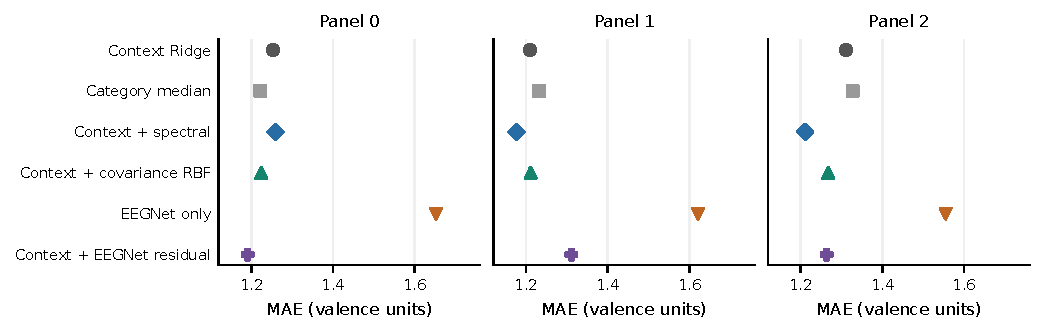
\includegraphics[width=\textwidth]{figures/mae_comparison.pdf}
\caption{Held-title development MAE for contextual and EEG-dependent predictors. The same twenty development participants and overlapping titles recur across rotations. Points are development results, not independent test estimates. Figure-generation code used OpenAI Codex assistance; plotted values were checked against public result packets. Exact model/version and human review require author confirmation.}
\label{fig:mae}
\end{figure}

Joint covariance RBF improves on matched context RBF by 0.0678, but by only 0.0238 against stronger context Ridge; its mean MAE exceeds spectral joint Ridge's. All three matched kernel descriptive intervals include zero. Reporting only the weaker comparator would overstate the incremental result.

EEGNet-only selects learning rate 0.001 and epoch 30; the residual model selects 0.003 and epoch 120. EEGNet-only is worse than the strongest EEG-free control in every rotation. Residual gains against the retrospective five-control minimum are \(+0.0314\), \(-0.1011\) and \(+0.0473\), averaging \(-0.0075\). That minimum is a post-hoc benchmark, not a source-selected deployable predictor. The residual model's mean MAE is close to context Ridge, but its improvements are inconsistent.

Source fitting and transfer differ. Joint covariance Ridge attains mean source MAE 0.255 but participant-excluded source error 1.778. At very low kernel regularization, spectral and covariance representations nearly interpolate both real and shuffled source targets; this does not imply prediction of held people. Five of six selected neural rotation/readout panels show over 10\% source-MSE improvement from epochs 60 to 120. Consequently, the fixed schedule does not establish optimized EEGNet performance.

Completed numerical audits reconstruct predictions, fallbacks, clipping, ensembles, selection and learning flags. Source-window/QC replay covers all 980 source and 265 available development trials. State-dictionary checks authenticate sixty checkpoints but do not constitute independent checkpoint-to-waveform forward replay. This manuscript adds no fitting or outcome access.

\subsection*{Interpretation}
The useful empirical observation is that supplied context provides a strong comparator under this inference contract. EEG-only and incremental EEG questions should be reported separately. Small joint-model differences depend on the comparator and material panel, while incomplete neural convergence limits a broad model-ranking conclusion. Acquisition fallback preserves assessment coverage without claiming artifact-free signals.

The practical implication is to report metadata controls, material grouping, trial availability and source-learning diagnostics together. This case study extends established confound and affect-regression work through a specific continuous retrospective target and simultaneous participant/title separation. It provides neither a confirmed method advantage nor a general EEG-information null.

\section*{Limitations}
All scores use adaptive development outcomes. Ridge choices use held-title validation, neural schedules use rotation 0, and earlier results informed the programme. Fixed later schedules do not make the overlapping rotations independent tests. Bootstrap intervals omit selection uncertainty.

Each unfamiliar panel contains six titles and no held-out Fear/Inspiration material. Additional people or windows cannot substitute for independent stimuli \cite{westfall2014power}. Catalogue grouping does not authenticate physical footage independence. A future confirmation must freeze a recipe, comparator and analysis before accessing reserved outcomes.

Whole-clip retrospective valence is not momentary affect. Marker-relative windows lack authenticated scene alignment or playback-latency calibration; rating reliability is unestablished. The context contract assumes assigned category and acquisition metadata at inference. These results do not directly transfer to deployments without that information. Whole-trial fallback may discard usable channels. The tested representations and fixed training budgets do not cover all modern EEG methods, and no matched foundation-model baseline is reported.
% MAIN_WORDCOUNT_END

\section*{Abbreviations}
EEG: electroencephalography; MAE: mean absolute error; MSE: mean squared error; OOF: out-of-fold; RBF: radial basis function.

\section*{Declarations}
\subsection*{Ethics approval and consent to participate}
This is a secondary analysis of existing FACED recordings; no new recordings or participant recruitment were undertaken. The dataset publication reports approval by the Tsinghua University Ethics Committee (THU201906) and informed consent from all participants \cite{chen2023faced}; it does not specify whether consent was written. \textbf{Pending author confirmation:} applicable institutional requirements for this secondary analysis, the venue's written-consent requirement and the final ethics statement. No new approval or exemption is asserted in this draft.

\subsection*{Consent for publication}
\textbf{Pending author confirmation.} The reported artifacts contain anonymous participant identifiers and aggregate or trial-level numerical predictions, without original recordings or identifiable images. The required publication-consent declaration must be confirmed before submission.

\subsection*{Availability of data and materials}
Original FACED data and author code are available through its Synapse project \cite{chen2023faced,faced2023release}. Analysis code, declared protocols, anonymous development predictions, complete candidate results and numerical audit receipts are available in the public repository \cite{analysisrepo2026}. The scientific packets used here are bound to repository revision \texttt{249f5fa161e4}; Additional file 1 maps their locations. Original recordings, stimuli and author archives are not redistributed. Reserved numerical outcomes are not included.

\subsection*{Competing interests}
\textbf{Pending confirmation from both authors.} No competing-interest declaration has been inferred.

\subsection*{Funding}
\textbf{Pending author confirmation.} Funding sources, grant identifiers and funder roles, or a confirmed absence of funding, must be supplied before submission.

\subsection*{Authors' contributions}
\textbf{Pending agreement by both authors.} Individual contributions and approval of the final manuscript must be confirmed; no roles have been assigned in this draft.

\subsection*{Acknowledgements and assistance disclosure}
OpenAI Codex was used for assistance with analysis-code preparation, experiment orchestration, literature checks, numerical/document audits and manuscript drafting. The scientific comparison figure was generated deterministically in Python from audited public summaries; no generative imagery was used. \textbf{Pending author review:} final verification of this disclosure, acknowledgements, factual content and conclusions. The author confirmed the order Muhammad Muntazar, then Muhammad Wasif Shakeel. Current affiliation, emails, corresponding author and exact AI model/version still require confirmation. Authors retain responsibility for the submitted manuscript; completed author approval is not asserted in this review copy.

\subsection*{Additional files}
Additional file 1: Detailed methods, complete results and evidence map (\nolinkurl{faced_supplementary_methods.pdf}).

Additional file 2: Machine-readable held-title development MAE table (\texttt{results\_table.csv}), covering fifteen declared conditions and the explicitly retrospective context benchmark.

\bibliographystyle{vancouver}
\bibliography{references}
\end{document}
